% THIS IS AN EXAMPLE DOCUMENT FOR VLDB 2012
% based on ACM SIGPROC-SP.TEX VERSION 2.7
% Modified by  Gerald Weber <gerald@cs.auckland.ac.nz>
% Removed the requirement to include *bbl file in here. (AhmetSacan, Sep2012)
% Fixed the equation on page 3 to prevent line overflow. (AhmetSacan, Sep2012)

\documentclass{vldb}
\usepackage{graphicx}
\usepackage{balance}  % for  \balance command ON LAST PAGE  (only there!)
\usepackage{xspace}
\usepackage{url}
\newcommand{\vispilot}{\textsc{VisPilot}\xspace}
\newcommand{\stitle}[1]{\par\noindent\textbf{#1}}

% Comments 
\newcommand{\agp}[1]{\leavevmode\textcolor[HTML]{AFCD38}{Aditya: #1}}
\newcommand{\dor}[1]{\leavevmode\textcolor[HTML]{00E8D8}{Doris: #1}}
\newcommand{\hdev}[1]{\leavevmode\textcolor[HTML]{9B6191}{Himel: #1}}
\newcommand{\haz}[1]{\leavevmode\textcolor[HTML]{E59400}{Hazem: #1}}

\urlstyle{leo}
% Include information below and uncomment for camera ready
\vldbTitle{A Sample Proceedings of the VLDB Endowment Paper in LaTeX Format}
\vldbAuthors{Ben Trovato, G. K. M. Tobin, Lars Th{\sf{\o}}rv{$\ddot{\mbox{a}}$}ld, Lawrence P. Leipuner, Sean Fogarty, Charles Palmer, John Smith, Julius P.~Kumquat, and Ahmet Sacan}
\vldbDOI{https://doi.org/10.14778/xxxxxxx.xxxxxxx}
\vldbVolume{12}
\vldbNumber{xxx}
\vldbYear{2019}

\begin{document}

% ****************** TITLE ****************************************

\title{VisPilot: Navigating Through Data Subsets with Hierarchical Summary of Visualizations}

\numberofauthors{5} 
\author{
       \alignauthor
       Doris Jung-Lin Lee\\
       \affaddr{University of Illinois}\\
       \email{jlee782@illinois.edu}
       \alignauthor
       Himel Dev\\
       \affaddr{University of Illinois}\\
       \email{hdev3@illinois.edu}
       \alignauthor
       Huizi Hu\\
       \affaddr{University of Illinois}\\
       \email{huizihu2@illinois.edu}
       \and  
       \alignauthor
       Hazem Elmeleegy\\
       \affaddr{Google Inc.}\\
       \email{elmeleegy@google.com}
       \alignauthor
       Aditya Parameswaran\\
       \affaddr{University of Illinois}\\
       \email{adityagp@illinois.edu}
}

% \author{Doris Jung-Lin Lee$^\dagger$, Himel Dev$^\dagger$, Huizi Hu$^\dagger$, Hazem Elmeleegy$^\star$, Aditya Parameswaran$^\dagger$}
% \renewcommand{\shortauthors}{D. Lee, H. Dev, H. Hu, H. Elmeleegy, A. Parameswaran}
% \affiliation{
%   \institution{$^\dagger$University of Illinois, Urbana-Champaign, $^\star$Google, Inc.}
% }
% \email{jlee782|hdev3|huizihu2|adityagp@illinois.edu, elmeleegy@google.com}

% There's nothing stopping you putting the seventh, eighth, etc.
% author on the opening page (as the 'third row') but we ask,
% for aesthetic reasons that you place these 'additional authors'
% in the \additional authors block, viz.
% \additionalauthors{Additional authors: John Smith (The Th{\o}rv\"{a}ld Group, {\texttt{jsmith@affiliation.org}}), Julius P.~Kumquat
% (The \raggedright{Kumquat} Consortium, {\small \texttt{jpkumquat@consortium.net}}), and Ahmet Sacan (Drexel University, {\small \texttt{ahmetdevel@gmail.com}})}
% \date{30 July 1999}
% Just remember to make sure that the TOTAL number of authors
% is the number that will appear on the first page PLUS the
% number that will appear in the \additionalauthors section.


\maketitle

\begin{abstract}
The abstract for your paper for the PVLDB Journal submission.
The template and the example document are based on the ACM SIG Proceedings  templates. This file is part of a package for preparing the submissions for review. These files are in the camera-ready format, but they do not contain the full copyright note.
Note that after the notification of acceptance, there will be an updated style file for the camera-ready submission containing the copyright note.
\end{abstract}

\section{Introduction}
Visual data exploration are accessible and intuitive means for helping analysts understand multidimensional datasets. Analysts often study data distributions at different levels of data granularity~\cite{Anand2015,Wu2013,Heer2012} to discover trends and patterns, generate or verify hypotheses, and understand complex causal relationships. While visualizations exploits analysts's perceptual capabilities for visual pattern recognition, the effectiveness of human perceptual reasoning breaks down as datasets increases in size and complexity. 
\par Manual exploration of multidimensional dataset is a time-consuming and error-prone process. To explore different subsets of data in a multidimensional dataset, an analysts would need to manually perform \emph{drill-downs} on the space of possible data subsets by adding one filter at a time, without knowing what data subset would lead to an insight. Even if visualizations for all possible data subsets has been constructed, there is no systematic way for analysts to make sense of or even navigate through this large space of possible visualizations. More alarmingly, without being able to contextualize the relationships between data subsets, analysts may mistaken the general cause of an observed deviation in trend for a specific cause---a fallacy coined as ``drill-down fallacy'' in our paper~\cite{Lee2019}.
\par To this end, we present \vispilot, a visual analytic tool that addresses the challenges of manual drill-down exploration. \vispilot traverses the space of possible data subsets (hereafter known as the \emph{lattice}) to \emph{automatically} identify a \emph{compact} network of  \emph{informative} and  \emph{interesting} visualizations that collectively convey the key insights in a dataset. Demo attendees will have the opportunity to interact with \vispilot to better understand and gain insights regarding of multiple provided datasets.
\section{Demonstration Scenario}


% subpopulation 
% pursue their own line of inquiry, expansion
\section{System}
\subsection{Recommendation Objective}
\subsection{System Design}
\vispilot is a web application built on top of a traditional in-memory database, PostgresSQL. Given a set of user selection via the frontend interface, the Interaction Manager relays the corresponding HTTP request to the Java backend. The backend runs within an embedded Jetty web-server and is responsible for managing the lattice (Lattice Manager) and querying data distributions for specified data subsets (Query Manager). The lattice manager consists of three modules: 1) construction of the lattice, 2) storage the lattice for subsequent reuse, and 3) traversal across the lattice in search of a maximal subgraph. Amongst the three modules, lattice construction is the most computationally intensive step, since the size of the lattice grows exponentially with the cardinality (across all attributes) in the dataset. \vispilot employs several optimization to ensure that the system generates a dashboard at interactive speeds.
\begin{enumerate}
	\item Instead of sending large numbers of independent database queries for every single data subset, the Query Manager applies sharing-based optimizations from Vartak et al.~\cite{Vartak2015}, submitting only a single query to the RDBMS via the Database Communicator and combining multiple aggregates to obtain the aggregate values for the requested subset.
	\item When generating the lattice combinatorially, we apply an early stopping criterion that limits the lattice to be no larger than 4 levels (default setting, further adjustable by users). This shell-fragment approach \cite{Li2004} is based on the observation that most analysts are only interested in data subsets with small numbers of filters, beyond that the filter becomes difficult to interpret. %The level cutoff parameter is adjustable by users if needed. 
	\item To eliminate insignificant subsets with small population sizes, users can also select an \textit{iceberg condition}~\cite{Xin2007} to adjust the extent of pruning on visualizations whose sizes fall below a certain percentage of the overall population size. %\footnote{The terminology is used in the discussion of iceberg cubes in OLAP literature. This also serves as a early pruning condition
\end{enumerate}
After the lattice is materialized, we cache the generated lattice both in-memory and in the database to facilitate further reuse. Upon a new dashboard request, \vispilot first performs a lookup in the Storage Module to see if a corresponding lattice has been generated for the selected set of \{Dataset, x,y, aggregation function\}. This ensures that dashboard refinement operations that requires low-latency, such as changing the number of requested dashboard (k) or requesting for a dashboard expansion, does not require lattice recomputation. The traversal module operates on top of the materialized lattice to search for the maximal weighted subgraph, via the fontier-greedy algorithm described in our paper~\cite{Lee2019}. Finally, the recommended subgraph is sent to the frontend in a JSON format. The Dashboard Renderer generates the recommended visualizations through Vega-Lite\footnote{\url{https://vega.github.io/vega-lite/}} and displays the visualizations in a connected graph layout through vis.js \footnote{\url{http://visjs.org/}}. 
\begin{figure}[ht!]
\centering
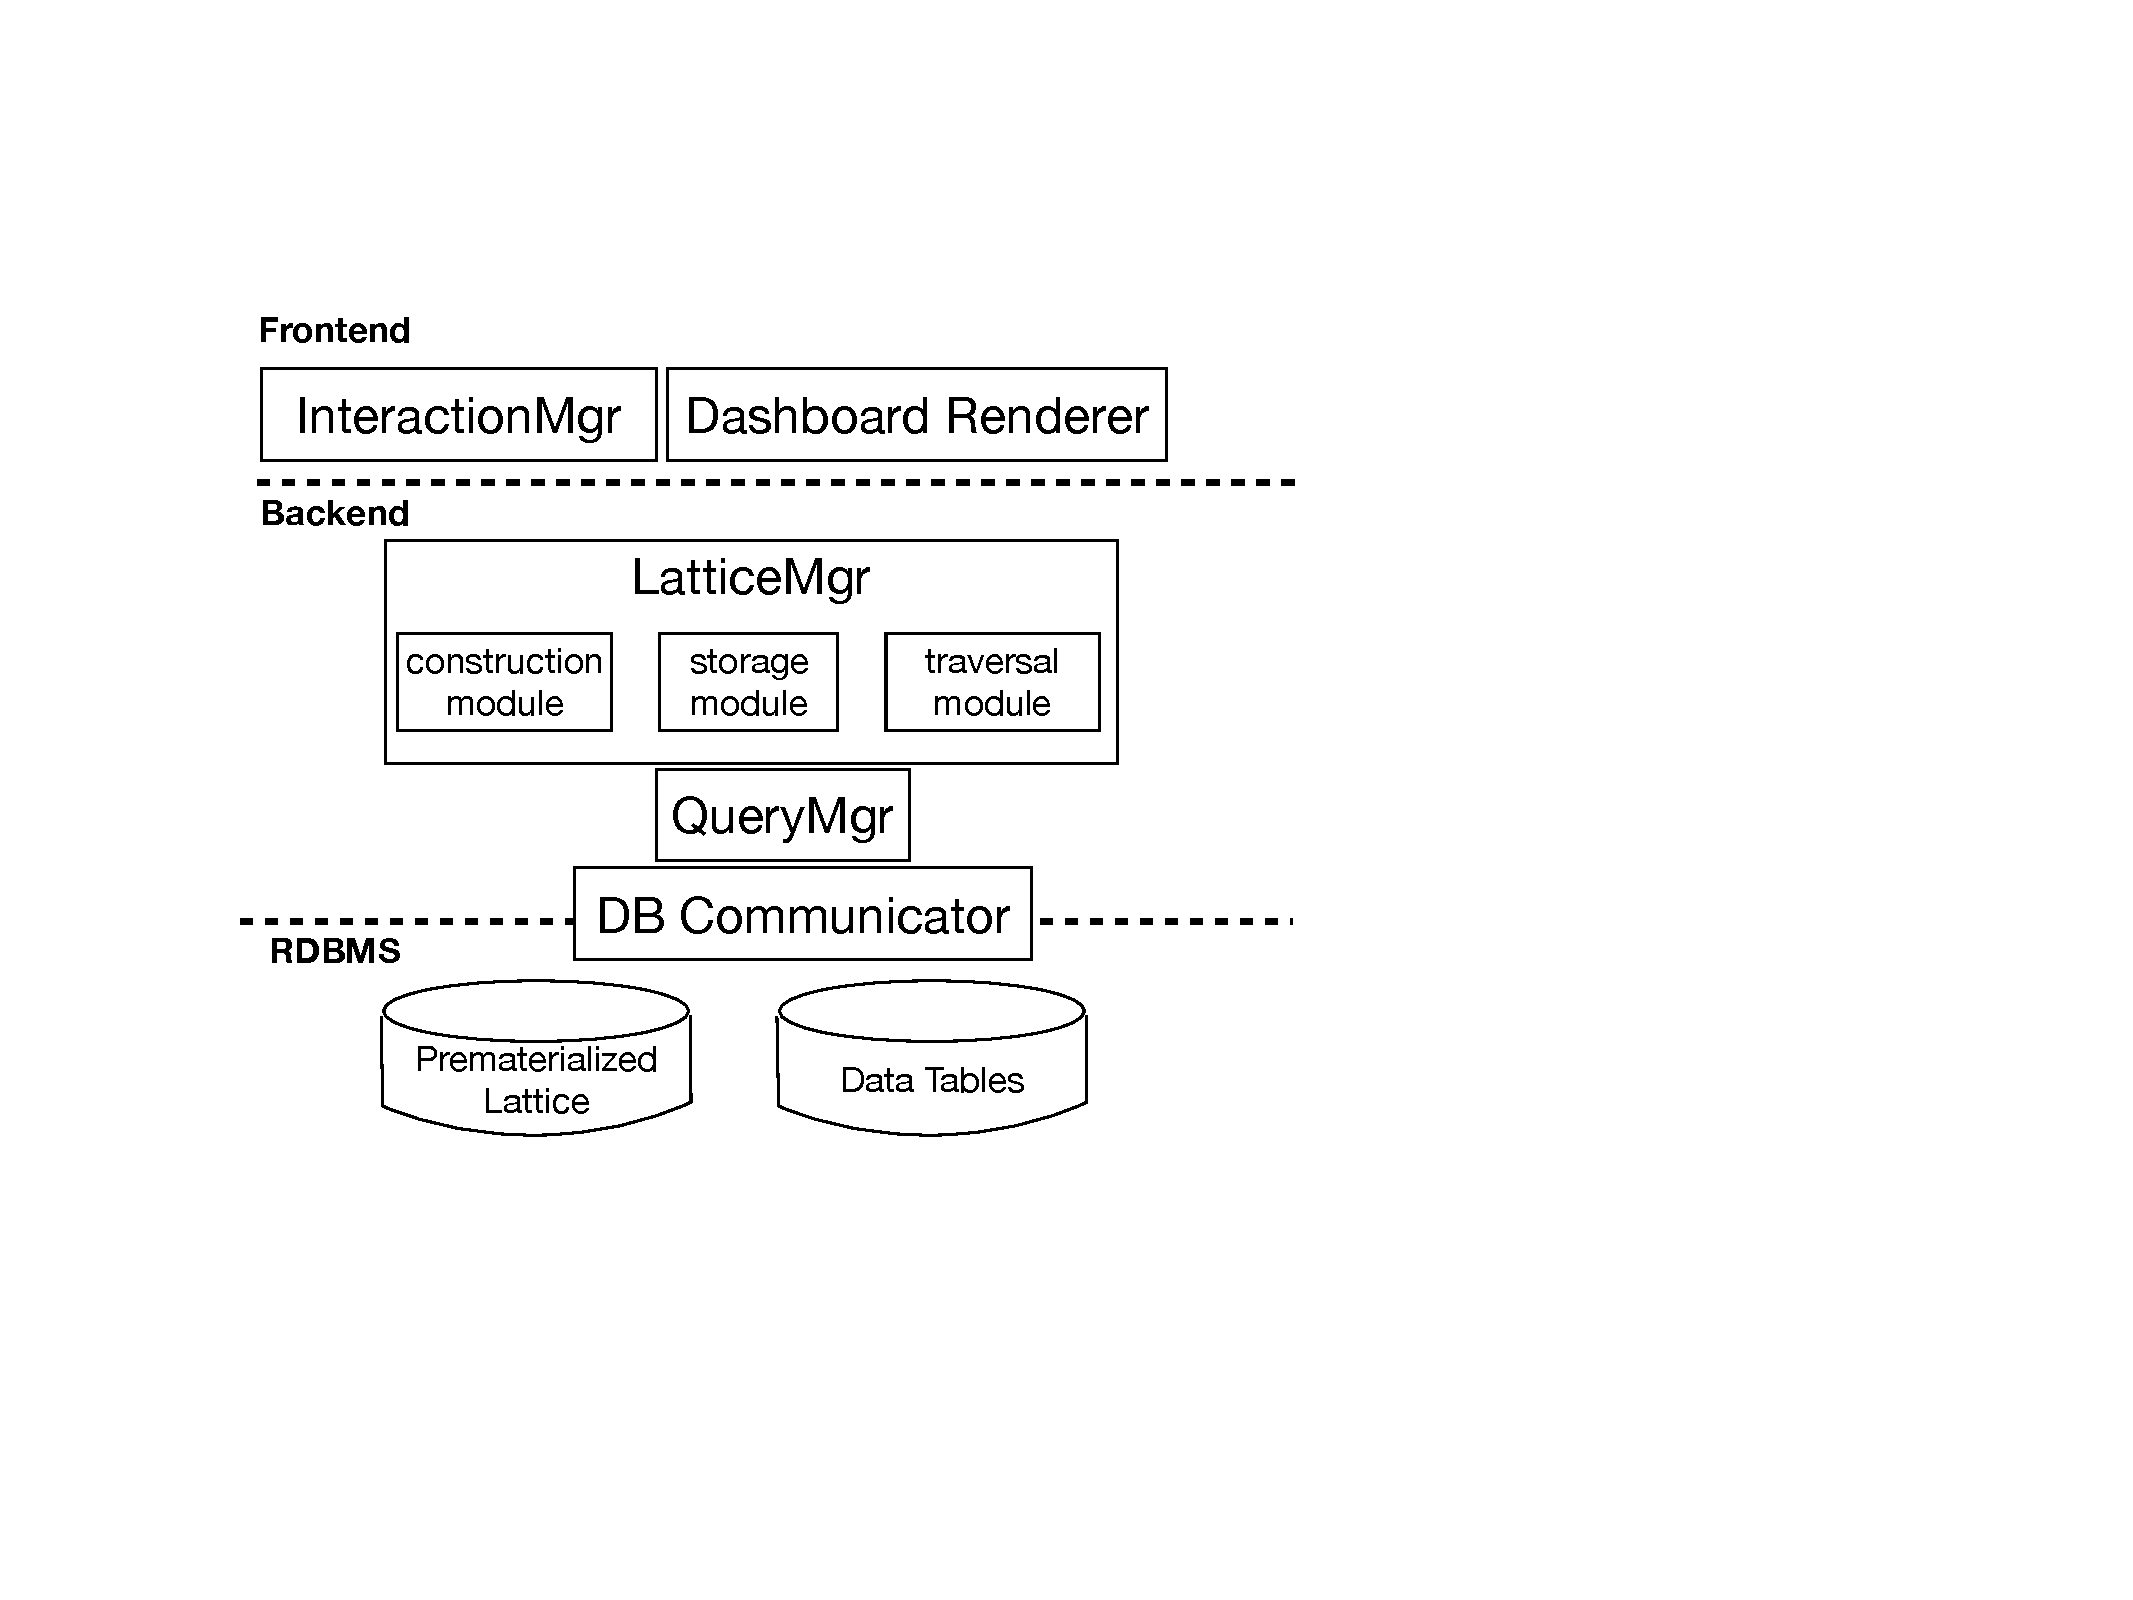
\includegraphics[width=0.9\linewidth]{figures/architecture.pdf}
\caption{\vispilot System Architecture}
% Default values are set for system related parameters such as the number of visualizations to show in the dashboard (k), iceberg condition for pruning ($\delta$), and informative parent criterion ($\theta$), which can be adjusted by the users via the sliders if needed.
\label{fig:architecture}
\vspace{-10pt}
\end{figure}

% when the backend retreives the aggregated data values from the database through SQL. 

% In most cases, the lattice contains a large number of visualizations due to the presence of many attributes or high-cardinality attributes in the dataset. In such cases finding an optimal solution is computationally challenging.
%  ---- There are several system optimizations 



% communicating with the database, managing and constructing the lattice, as well as traversing through the lattice in search of the recommendation. First, the backend retreives the aggregated data values from the database through SQL. The data values are used to construct the lattice combinatorially in a level-wise order. 

% - lattice construction 
% - traversal modules
% visualization rendered using Vega-Lite\footnote{\url{https://vega.github.io/vega-lite/}}
% Frontend: 
% 	- handles requests
% 	- graph layout through vis.js \footnote{\url{http://visjs.org/}}
%     - communication through HTTP request




%Our system supports two variants of traversal based on the lattice generation procedure---offline variants that first generate the complete lattice and then work towards identifying the solution with maximum combined-edge utility, and online variants that incrementally generate the lattice and simultaneously identify the solution. The offline variants are appropriate for datasets with a small number of low-cardinality attributes, where we can generate the entire lattice in a reasonable time; whereas the online variants are appropriate for datasets with many high-cardinality attributes, where we need to incrementally generate a partial lattice. 




\section{Conclusion}
% ensure same length columns on last page (might need two sub-sequent latex runs)
\balance

%ACKNOWLEDGMENTS are optional
\medskip
\stitle{Acknowledgments.} We thank the anonymous reviewers for their valuable feedback. We acknowledge support from grants IIS-1513407, IIS-1633755, IIS-1652750, and IIS-1733878 awarded by the National Science Foundation, and funds from Microsoft, 3M, Adobe, Toyota Research Institute, Google, and the Siebel Energy Institute. The content is solely the responsibility of the authors and does not necessarily represent the official views of the funding agencies and organizations.
% \section{Acknowledgments}
% This section is optional; it is a location for you
% to acknowledge grants, funding, editing assistance and
% what have you.  In the present case, for example, the
% authors would like to thank Gerald Murray of ACM for
% his help in codifying this \textit{Author's Guide}
% and the \textbf{.cls} and \textbf{.tex} files that it describes.
\bibliographystyle{abbrv}
\bibliography{reference}  % vldb_sample.bib is the name of the Bibliography in this case
\end{document}
